\subsubsection{BaseWidgetView}

\label{BaseWidgetView}
\begin{figure}[ht]
	\centering
	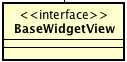
\includegraphics[scale=0.5]{Sezioni/SottosezioniST/img/BaseWidgetView.png}
	\caption{BaseWidgetView}
\end{figure}

\begin{itemize}
\item \textbf{Descrizione:} Interfaccia che estende BaseComponent che rappresenta un qualsiasi widget che può essere inserito all'interno di un bolla.
\item \textbf{Utilizzo:} Interfaccia che viene utilizzata ed implementata ogniqualvolta uno sviluppatore intende aggiungere widget.
\item \textbf{Attributi:}
\item \textbf{Metodi:}
\end{itemize}

\subsubsection{ButtonWidgetView}

\label{ButtonWidgetView}
\begin{figure}[ht]
	\centering
	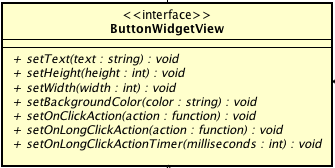
\includegraphics[scale=0.5]{Sezioni/SottosezioniST/img/ButtonWidgetView.png}
	\caption{ButtonWidgetView}
\end{figure}

\begin{itemize}
\item \textbf{Descrizione}: Questa interfaccia rappresenta la view relativa ai widget di tipo bottone.
\item \textbf{Utilizzo}: L'interfaccia viene utilizzata per disaccoppiare presenter e implementazione del widget, visualizza i dati che gli vengono passati dal presenter.
\item \textbf{Attributi}:
\item \textbf{Metodi}:
	\begin{itemize}
	\item \textit{public setText(string text:int):void}\\
	Imposta il testo all'interno del bottone.
		\item{\textbf{Parametri}: \begin{itemize}
		\item \textit{text:string:int}\\
		Rappresenta il testo che verrà impostato all'interno del bottone.
		\end{itemize}}
	\item \textit{public setHeight(height:int):void}\\
	Imposta l'altezza del bottone.
		\item{\textbf{Parametri}: \begin{itemize}
		\item \textit{height:int}\\
		Rappresenta il numero di pixel corrispondente all'altezza del bottone che verrà impostata.
		\end{itemize}}
	\item \textit{public setWidth(width:int):void}\\
	Imposta la larghezza del bottone.
		\item{\textbf{Parametri}: \begin{itemize}
		\item \textit{width:int}\\
		Rappresenta il numero di pixel corrispondente alla larghezza del bottone che verrà impostata.
		\end{itemize}}
	\item \textit{public setBackgroundColor(color:string):void}\\
	Imposta il colore di sfondo del bottone.
		\item{\textbf{Parametri}: \begin{itemize}
		\item \textit{color:string}\\
		Rappresenta la stringa in esadecimale corrispondente al colore che verrà impostata come sfondo del bottone.
		\end{itemize}}
	\end{itemize}
\end{itemize}

\subsubsection{ButtonWidget}

\label{ButtonWidget}
\begin{figure}[ht]
	\centering
	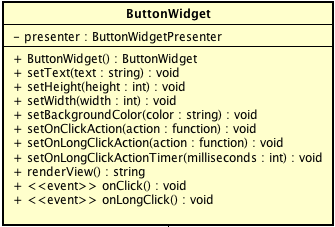
\includegraphics[scale=0.5]{Sezioni/SottosezioniST/img/ButtonWidget.png}
	\caption{ButtonWidget}
\end{figure}

\begin{itemize}
\item \textbf{Descrizione}: Questa classe rappresenta un widget buttone, implementando l'interfaccia ButtonWidgetView.
\item \textbf{Utilizzo}: Implementando i metodi di ButtonWidgetView questa classe viene utilizzata al momento della creazione e della personalizzazione del bottone e delle sue reazioni alle azioni degli utenti.
\item \textbf{Attributi}: 
	\begin{itemize}
	\item \textit{private presenter:ButtonWidgetPresenter}\\
	Il presenter associato al widget bottone, al quale questa classe delega la gestione del comportamento del widget stesso.
	\end{itemize}
\item \textbf{Metodi}:
	\begin{itemize}
	\item \textit{public renderView():string}\\
	 Genera il codice HTML CSS JS necessario per visualizzare il widget.
	\item \textit{public setText(string text:int):void}\\
	Imposta il testo all'interno del bottone.
		\item{\textbf{Parametri}: \begin{itemize}
		\item \textit{text:int}\\
		Rappresenta il testo che verrà impostato all'interno del bottone.
		\end{itemize}}
	\item \textit{public setHeight(height:int):void}\\
	Imposta l'altezza del bottone.
		\item{\textbf{Parametri}: \begin{itemize}
		\item \textit{height:int}\\
		Rappresenta il numero di pixel corrispondente all'altezza del bottone che verrà impostata.
		\end{itemize}}
	\item \textit{public setWidth(width:int):void}\\
	Imposta la larghezza del bottone.
		\item{\textbf{Parametri}: \begin{itemize}
		\item \textit{width:int}\\
		Rappresenta il numero di pixel corrispondente alla larghezza del bottone che verrà impostata.
		\end{itemize}}
	\item \textit{public setBackgroundColor(color:string):void}\\
	Imposta il colore di sfondo del bottone.
		\item{\textbf{Parametri}: \begin{itemize}
		\item \textit{color:string}\\
		Rappresenta la stringa in esadecimale corrispondente al colore che verrà impostata come sfondo del bottone.
		\end{itemize}}
	\end{itemize}
\item{Eventi}
	\begin{itemize}
	\item \textit{public onClick():void}\\
	Evento che rappresenta il click normale sul bottone, dopo il quale si può personalizzare la reazione del bottone.
	\item \textit{public onLongClick():void}\\
	Evento che rappresenta il click prolungato sul bottone, dopo il quale si può personalizzare la reazione del bottone.
	\end{itemize}
\end{itemize}

\subsubsection{ButtonWidgetPresenter}

\label{ButtonWidgetPresenter}
\begin{figure}[ht]
	\centering
	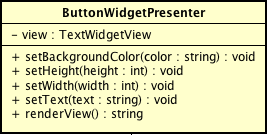
\includegraphics[scale=0.5]{Sezioni/SottosezioniST/img/ButtonWidgetPresenter.png}
	\caption{ButtonWidgetPresenter}
\end{figure}

\begin{itemize}
\item \textbf{Descrizione}: Questa classe rappresenta il presenter per i widget di tipo bottone.
\item \textbf{Utilizzo}: Il presenter fa da tramite tra l'implementazione del widget e la view, formattando i dati che verranno visualizzati nella view.
\item \textbf{Attributi}:
	\begin{itemize}
	\item \textit{private view:ButtonWidgetView}\\
	La view associata al presenter.
	\end{itemize}
\item \textbf{Metodi}:
	\begin{itemize}
	\item \textit{public setText(string text:int):void}\\
	Imposta il testo all'interno del bottone
		\item{\textbf{Parametri}: \begin{itemize}
		\item \textit{text:string:int}\\
		Rappresenta il testo che verrà impostato all'interno del bottone.
		\end{itemize}}
	\item \textit{public setHeight(height:int):void}\\
	Imposta l'altezza del bottone.
		\item{\textbf{Parametri}: \begin{itemize}
		\item \textit{height:int}\\
		Rappresenta il numero di pixel corrispondente all'altezza del bottone che verrà impostata.
		\end{itemize}}
	\item \textit{public setWidth(width:int):void}\\
	Imposta la larghezza del bottone.
		\item{\textbf{Parametri}: \begin{itemize}
		\item \textit{width:int}\\
		Rappresenta il numero di pixel corrispondente alla larghezza del bottone che verrà impostata.
		\end{itemize}}
	\item \textit{public setBackgroundColor(color:string):void}\\
	Imposta il colore di sfondo del bottone.
		\item{\textbf{Parametri}: \begin{itemize}
		\item \textit{color:string}\\
		Rappresenta la stringa in esadecimale corrispondente al colore che verrà impostata come sfondo del bottone.
		\end{itemize}}
	\item \textit{public renderView():string}\\
	Genera il codice HTML CSS JS necessario per visualizzare il widget.
	\end{itemize}
\end{itemize}

\subsubsection{ButtonGraphics}

\label{ButtonGraphics}
\begin{figure}[ht]
	\centering
	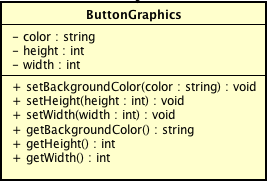
\includegraphics[scale=0.5]{Sezioni/SottosezioniST/img/ButtonGraphics.png}
	\caption{ButtonGraphics}
\end{figure}

\begin{itemize}
\item \textbf{Descrizione}: Questa classe rappresenta l'aspetto visivo del bottone.
\item \textbf{Utilizzo}:
\item \textbf{Attributi}:
	\begin{itemize}
	\item \textit{private color:string}\\
	Rappresenta la stringa in esadecimale corrispondente al colore che verrà impostata come sfondo del bottone.
	\item \textit{private height:int}\\
	Rappresenta il numero di pixel corrispondente all'altezza del bottone. 
	\item \textit{private width:int}\\
	Rappresenta il numero di pixel corrispondente alla larghezza del bottone.
	\end{itemize}
\item \textbf{Metodi}:
	\begin{itemize}
	\item \textit{public setHeight(height:int):void}\\
	Imposta l'altezza del bottone.
		\item{\textbf{Parametri}: \begin{itemize}
		\item \textit{height:int}\\
		Rappresenta il numero di pixel corrispondente all'altezza del bottone che verrà impostata.
		\end{itemize}}
	\item \textit{public setWidth(width:int):void}\\
	imposta la larghezza del bottone.
		\item{\textbf{Parametri}: \begin{itemize}
		\item \textit{width:int}\\
		Rappresenta il numero di pixel corrispondente alla larghezza del bottone che verrà impostata.
		\end{itemize}}
	\item \textit{public setBackgroundColor(color:string):void}\\
	imposta il colore di sfondo del bottone.
		\item{\textbf{Parametri}: \begin{itemize}
		\item \textit{color:string}\\
		Rappresenta la stringa in esadecimale corrispondente al colore che verrà come sfondo del bottone.
		\end{itemize}}
	\item \textit{public getHeight():int}\\
	Ritorna l'altezza del bottone.
	\item \textit{public getWidth():int}\\
	Ritorna la larghezza del bottone.
	\item \textit{public getBackgroundColor():string}\\
	Ritorna la stringa in esadecimale corrispondente al colore di sfondo del bottone.
	\end{itemize}
\end{itemize}

\subsubsection{TextWidgetView}

\label{TextWidgetView}
\begin{figure}[ht]
	\centering
	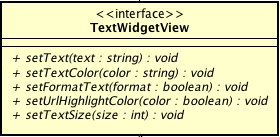
\includegraphics[scale=0.5]{Sezioni/SottosezioniST/img/TextWidgetView.png}
	\caption{TextWidgetView}
\end{figure}

\begin{itemize}
\item \textbf{Descrizione}: Questa interfaccia rappresenta la view relativa ai widget di tipo testo.
\item \textbf{Utilizzo}: L'interfaccia viene utilizzata per disaccoppiare presenter e implementazione del widget, visualizza i dati che gli vengono passati dal presenter.
\item \textbf{Attributi}:
\item \textbf{Metodi}:
	\begin{itemize}
	\item \textit{public setText(string text:int):void}\\
	Imposta il testo all'interno del widget testo.
		\item{\textbf{Parametri}: \begin{itemize}
		\item \textit{string text:int}\\
		Rappresenta con una string il testo che va inserito all'interno del widget.
		\end{itemize}}
	\item \textit{public setTextColor(color:string):void}\\
	Imposta il colore del testo del widget testo.
		\item{\textbf{Parametri}: \begin{itemize}
		\item \textit{color:string}\\
		Rappresenta la stringa in esadecimale corrispondente al colore che verrà come sfondo del bottone.
		\end{itemize}}
	\item \textit{public setFormatText(format: boolean):void}\\
	Imposta il widget a testo formattato o testo semplice.
		\item{\textbf{Parametri}: \begin{itemize}
		\item \textit{format: boolean}\\
		Questo booleano viene impostato a true se si vuole il testo del widget formattato, a false altrimenti.
		\end{itemize}}
	\item \textit{public setUrlHighlightColor(color:boolean):void}\\
	Imposta la possiblità di cliccare o meno i link presenti nel testo del widget.
		\item{\textbf{Parametri}: \begin{itemize}
		\item \textit{color:string}\\
		Questo booleano viene impostato a true se si vogliono i link cliccabili, a false altrimenti.
		\end{itemize}}
	\item \textit{public setTextSize(size:int):void}\\
	Imposta la grandezza del testo nel widget
		\item{\textbf{Parametri}: \begin{itemize}
		\item \textit{size:int}\\
		Rappresenta il numero di pixel corrispondente all'altezza del testo che verrà impostata all'interno del widget.
		\end{itemize}}
	\end{itemize}
\end{itemize}

\subsubsection{TextWidget}

\label{TextWidget}
\begin{figure}[ht]
	\centering
	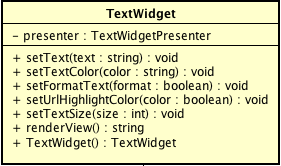
\includegraphics[scale=0.5]{Sezioni/SottosezioniST/img/TextWidget.png}
	\caption{TextWidget}
\end{figure}

\begin{itemize}
\item \textbf{Descrizione}: Questa classe rappresenta un widget di testo, implementando l'interfaccia TextWidgetView
\item \textbf{Utilizzo}: Implementando i metodi di TextWidgetView questa classe viene utilizzata al momento della creazione e della personalizzazione del widget di testo e del suo contenuto.
\item \textbf{Attributi}:
	\begin{itemize}
	\item \textit{private presenter:TextWidgetPresenter}\\
	Il presenter associato al widget testo, al quale questa classe delega la gestione del comportamento del widget stesso.
	\end{itemize}
\item \textbf{Metodi}:
	\begin{itemize}
	\item \textit{public setText(string text:int):void}\\
	Imposta il testo all'interno del widget testo.
		\item{\textbf{Parametri}: \begin{itemize}
		\item \textit{string text:int}\\
		Rappresenta con una string il testo che va inserito all'interno del widget.
		\end{itemize}}
	\item \textit{public setTextColor(color:string):void}\\
	Imposta il colore del testo del widget testo.
		\item{\textbf{Parametri}: \begin{itemize}
		\item \textit{color:string}\\
		Rappresenta la stringa in esadecimale corrispondente al colore che verrà come sfondo del bottone.
		\end{itemize}}
	\item \textit{public setFormatText(format: boolean):void}\\
	Imposta il widget a testo formattato o testo semplice.
		\item{\textbf{Parametri}: \begin{itemize}
		\item \textit{format: boolean}\\
		Questo booleano viene impostato a true se si vuole il testo del widget formattato, a false altrimenti.
		\end{itemize}}
	\item \textit{public setUrlHighlightColor(color:boolean):void}\\
	Imposta la possiblità di cliccare o meno i link presenti nel testo del widget.
		\item{\textbf{Parametri}: \begin{itemize}
		\item \textit{color:string}\\
		Questo booleano viene impostato a true se si vogliono i link cliccabili, a false altrimenti.
		\end{itemize}}
	\item \textit{public setTextSize(size:int):void}\\
	Imposta la grandezza del testo nel widget
		\item{\textbf{Parametri}: \begin{itemize}
		\item \textit{size:int}\\
		Rappresenta il numero di pixel corrispondente all'altezza del testo che verrà impostata all'interno del widget.
		\end{itemize}}
	\item \textit{public renderView():string}\\
	Genera il codice HTML CSS JS necessario per visualizzare il widget.
	\end{itemize}
\end{itemize}

\subsubsection{TextWidgetPresenter}

\label{TextWidgetPresenter}
\begin{figure}[ht]
	\centering
	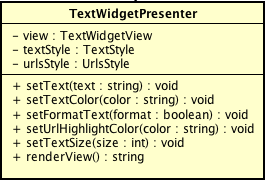
\includegraphics[scale=0.5]{Sezioni/SottosezioniST/img/TextWidgetPresenter.png}
	\caption{TextWidgetPresenter}
\end{figure}

\begin{itemize}
\item \textbf{Descrizione}: Questa classe rappresenta il presenter per i widget di tipo testo.
\item \textbf{Utilizzo}: Il presenter fa da tramite tra l'implementazione del widget e la view,  formattando i dati che verranno visualizzati nella view.
\item \textbf{Attributi}:
	\begin{itemize}
	\item \textit{private view:TextWidgetView}\\
	La view associata al presenter.
	\item \textit{private textStyle:TextStyle}\\
	Stile del testo del widget.
	\item \textit{private urlsStyle:UrlsStyle}\\
	Stile dei link presenti all'interno del testo.
	\end{itemize}
\item \textbf{Metodi}:
	\begin{itemize}
	\item \textit{public setText(string text:int):void}\\
	Imposta il testo all'interno del widget testo.
		\item{\textbf{Parametri}: \begin{itemize}
		\item \textit{string text:int}\\
		Rappresenta con una string il testo che va inserito all'interno del widget.
		\end{itemize}}
	\item \textit{public setTextColor(color:string):void}\\
	Imposta il colore del testo del widget testo.
		\item{\textbf{Parametri}: \begin{itemize}
		\item \textit{color:string}\\
		Rappresenta la stringa in esadecimale corrispondente al colore che verrà impostato al testo all'interno del widget.
		\end{itemize}}
	\item \textit{public setFormatText(format: boolean):void}\\
	Imposta il widget a testo formattato o testo semplice.
		\item{\textbf{Parametri}: \begin{itemize}
		\item \textit{format: boolean}\\
		Questo booleano viene impostato a true se si vuole il testo del widget formattato, a false altrimenti.
		\end{itemize}}
	\item \textit{public setUrlHighlightColor(color:boolean):void}\\
	Imposta la possiblità di cliccare o meno i link presenti nel testo del widget.
		\item{\textbf{Parametri}: \begin{itemize}
		\item \textit{color:string}\\
		Questo booleano viene impostato a true se si vogliono i link cliccabili, a false altrimenti.
		\end{itemize}}
	\item \textit{public setTextSize(size:int):void}\\
	Imposta la grandezza del testo nel widget.
		\item{\textbf{Parametri}: \begin{itemize}
		\item \textit{size:int}\\
		Rappresenta il numero di pixel corrispondente all'altezza del testo che verrà impostata all'interno del widget.
		\end{itemize}}
	\item \textit{public renderView():string}\\
	Genera il codice HTML CSS JS necessario per visualizzare il widget.
	\end{itemize}
\end{itemize}

\subsubsection{TextStyle}

\label{TextStyle}
\begin{figure}[ht]
	\centering
	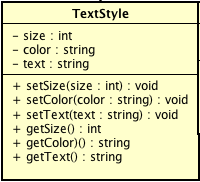
\includegraphics[scale=0.5]{Sezioni/SottosezioniST/img/TextStyle.png}
	\caption{TextStyle}
\end{figure}

\begin{itemize}
\item \textbf{Descrizione}: Questa classe rappresenta lo stile del testo all'interno di un widget testo.
\item \textbf{Utilizzo}:
\item \textbf{Attributi}:
	\begin{itemize}
	\item \textit{private size:int}\\
	Rappresenta il numero di pixel corrispondente all'altezza del testo.
	\item \textit{private color:string}\\
	Rappresenta la stringa in esadecimale corrispondente al colore del testo.
	\item \textit{private text:string}\\
	Rappresenta il testo stesso. 
	\end{itemize}
\item \textbf{Metodi}:
	\begin{itemize}
	\item \textit{public setSize(size:int):void}\\
	Imposta la grandezza del testo.
		\item{\textbf{Parametri}: \begin{itemize}
		\item \textit{size:int}\\
		Rappresenta il numero di pixel corrispondente all'altezza del testo che verrà impostata all'interno del widget.
		\end{itemize}}
	\item \textit{public setColor(color:string):void}\\
	Imposta il colore del testo del widget testo.
		\item{\textbf{Parametri}: \begin{itemize}
		\item \textit{color:string}\\
		Rappresenta la stringa in esadecimale corrispondente al colore che verrà impostato al testo all'interno del widget.
		\end{itemize}}
	\item \textit{public setText(string text:int):void}\\
	Imposta il testo.
		\item{\textbf{Parametri}: \begin{itemize}
		\item \textit{string text:int}\\
		Rappresenta con una string il testo che va inserito.
		\end{itemize}}
	\item \textit{public getSize():int}\\
	Ritorna il numero di pixel corrispondente all'altezza del testo.
	\item \textit{public getColor():string}\\
	Ritorna  la stringa in esadecimale corrispondente al colore del testo.
	\item \textit{public getText():string}\\
	Ritorna la stringa contenente il testo.
	\end{itemize}
\end{itemize}

\subsubsection{UrlStyle}

\label{UrlsStyle}
\begin{figure}[ht]
	\centering
	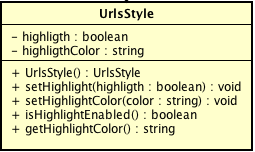
\includegraphics[scale=0.5]{Sezioni/SottosezioniST/img/UrlsStyle.png}
	\caption{UrlsStyle}
\end{figure}

\begin{itemize}
\item \textbf{Descrizione}: Questa classe rappresenta lo stile del testo dei link all'interno di un widget testo.
\item \textbf{Utilizzo}:
\item \textbf{Attributi}:
	\begin{itemize}
	\item \textit{private highlight:boolean}\\
	Booleano che rappresenta la possibilità o meno di cliccare i link nel testo.
	\item \textit{private highlightColor:string}\\
	Stringa in esadecimale corrispondente al colore dei link al testo all'interno del testo.
	\end{itemize}
\item \textbf{Metodi}:
	\begin{itemize}
	\item \textit{public setHighlight(color:boolean):void}\\
	Imposta la possiblità di cliccare o meno i link presenti nel testo.
		\item{\textbf{Parametri}: \begin{itemize}
		\item \textit{color:string}\\
		Questo booleano viene impostato a true se si vogliono i link cliccabili, a false altrimenti.
		\end{itemize}}
	\item \textit{public setHighlightColor(color:string):void}\\
	Imposta il colore del testo dei link presenti all'interno del testo.
		\item{\textbf{Parametri}: \begin{itemize}
		\item \textit{color:string}\\
		Rappresenta la stringa in esadecimale corrispondente al colore che verrà impostato per i link al testo all'interno del testo.
		\end{itemize}}
	\item \textit{public isHighlightEnabled():boolean}\\
	Ritorna true se i link sono cliccabili, false altrimenti.
	\item \textit{public getHighlightColor():string}\\
	Ritorna la stringa in esadecimale corrispondente al colore che verrà impostato per i link al testo all'interno del widget.
	\end{itemize}
\end{itemize}

\subsubsection{ChecklistWidgetView}

\label{ChecklistWidgetView}
\begin{figure}[ht]
	\centering
	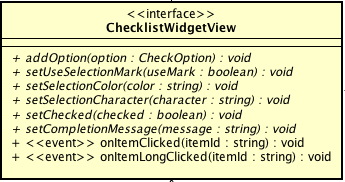
\includegraphics[scale=0.5]{Sezioni/SottosezioniST/img/ChecklistWidgetView.png}
	\caption{ChecklistWidgetView}
\end{figure}

\begin{itemize}
\item \textbf{Descrizione}: Questa interfaccia rappresenta la view relativa ai widget di tipo checklist.
\item \textbf{Utilizzo}: L'interfaccia viene utilizzata per disaccoppiare presenter e implementazione del widget, visualizza i dati che gli vengono passati dal presenter.
\item \textbf{Attributi}:
\item \textbf{Metodi}:
	\begin{itemize}
	\item \textit{public addOption(option:CheckOption):void}\\
	Questo metodo aggiunge una entry alla checklist.
		\item{\textbf{Parametri}: \begin{itemize}
		\item \textit{option:CheckOption}\\
		L'entry della checklist che verrà aggiunta.
		\end{itemize}}
	\item \textit{public setCheckStyle(style:CheckStyle):void}\\
	Questo metodo imposta lo stile per le spunte delle opzioni della checklist.
		\item{\textbf{Parametri}: \begin{itemize}
		\item \textit{style:CheckStyle}\\
		Lo stile per le spunte delle opzioni della checklist che verrà impostata.
		\end{itemize}} 
	\item \textit{public setCompletionMessage(message:string):void}\\
	Questo metodo imposta il messaggio di completamento che viene visualizzato quando tutte le opzioni della lista vengono spuntate.
		\item{\textbf{Parametri}: \begin{itemize}
		\item \textit{message:string}\\
		Stringa che rappresenta il messaggio di completamento della checklist.
		\end{itemize}}
	\end{itemize}
\item{Eventi}:
	\begin{itemize}
	\item \textit{public onClick():void}\\
	Evento che rappresenta il click normale, dopo il quale si può personalizzare la reazione della checklist.
	\item \textit{public onLongClick():void}\\
	Evento che rappresenta il click prolungato, dopo il quale si può personalizzare la reazione della checklist.
	\end{itemize}
\end{itemize}

\subsubsection{ChecklistWidget}

\label{ChecklistWidget}
\begin{figure}[ht]
	\centering
	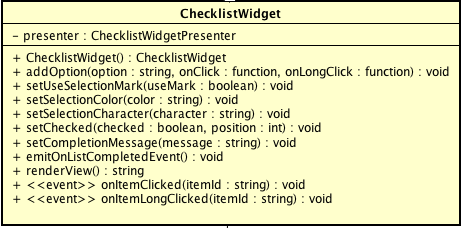
\includegraphics[scale=0.5]{Sezioni/SottosezioniST/img/ChecklistWidget.png}
	\caption{ChecklistWidget}
\end{figure}

\begin{itemize}
\item \textbf{Descrizione}: Questa classe rappresenta un widget checklist, implementando l'interfaccia ChecklistWidgetView
\item \textbf{Utilizzo}: Implementando i metodi di ChecklistWidgetView questa classe viene utilizzata al momento della creazione e della personalizzazione del widget checklist e del suo contenuto.
\item \textbf{Attributi}:
	\begin{itemize}
	\item \textit{private presenter:ChecklistWidgetPresenter}\\
	Il presenter associato al widget checklist, al quale questa classe delega la gestione del comportamento del widget stesso.
	\end{itemize}
\item \textbf{Metodi}:
	\begin{itemize}
	\item \textit{public addOption(option:CheckOption):void}\\
	Questo metodo aggiunge una entry alla checklist.
		\item{\textbf{Parametri}: \begin{itemize}
		\item \textit{option:CheckOption}\\
		L'entry della checklist che verrà aggiunta.
		\end{itemize}}
	\item \textit{public setCheckStyle(style:CheckStyle):void}\\
	Questo metodo imposta lo stile per le spunte delle opzioni della checklist.
		\item{\textbf{Parametri}: \begin{itemize}
		\item \textit{style:CheckStyle}\\
		Lo stile per le spunte delle opzioni della checklist che verrà impostata.
		\end{itemize}} 
	\item \textit{public setCompletionMessage(message:string):void}\\
	Questo metodo imposta il messaggio di completamento che viene visualizzato quando tutte le opzioni della lista vengono spuntate.
		\item{\textbf{Parametri}: \begin{itemize}
		\item \textit{message:string}\\
		Stringa che rappresenta il messaggio di completamento della checklist.
		\end{itemize}}
	\item \textit{public renderView():string}\\
	Genera il codice HTML CSS JS necessario per visualizzare il widget.
	\end{itemize}
\item{Eventi}:
	\begin{itemize}
	\item \textit{public onItemClicked(itemID:string):void}\\
	Evento che rappresenta il click normale su una delle entry della lista, dopo il quale si può personalizzare la reazione della checklist.
	\item \textit{public onItemLongClicked(itemId:string):void}\\
	Evento che rappresenta il click prolungato su una delle entry della lista, dopo il quale si può personalizzare la reazione della checklist.
	\end{itemize}
\end{itemize}

\subsubsection{ChecklistWidgetPresenter}

\label{ChecklistWidgetPresenter}
\begin{figure}[ht]
	\centering
	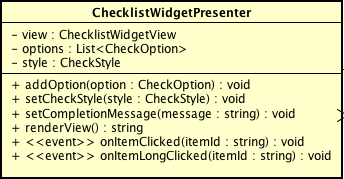
\includegraphics[scale=0.5]{Sezioni/SottosezioniST/img/ChecklistWidgetPresenter.png}
	\caption{ChecklistWidgetPresenter}
\end{figure}

\begin{itemize}
\item \textbf{Descrizione}: Questa classe rappresenta il presenter per i widget di tipo checklist.
\item \textbf{Utilizzo}: Il presenter fa da tramite tra l'implementazione del widget e la view, formattando i dati che verranno visualizzati nella view.
\item \textbf{Attributi}:
	\begin{itemize}
	\item \textit{private view:ChecklistWidgetView}\\
	La view associata al presenter.
	\item \textit{private options:List<CheckOption>}\\
	Collezione contentente tutte le opzioni della lista.
	\item \textit{private style:CheckStyle}\\
	Stile per le spunte della lista.
	\end{itemize}
\item \textbf{Metodi}:
	\begin{itemize}
	\item \textit{public addOption(option:CheckOption):void}\\
	Questo metodo aggiunge una entry alla checklist.
		\item{\textbf{Parametri}: \begin{itemize}
		\item \textit{option:CheckOption}\\
		L'entry della checklist che verrà aggiunta.
		\end{itemize}}
	\item \textit{public setCheckStyle(style:CheckStyle):void}\\
	Questo metodo imposta lo stile per le spunte delle opzioni della checklist.
		\item{\textbf{Parametri}: \begin{itemize}
		\item \textit{style:CheckStyle}\\
		Lo stile per le spunte delle opzioni della checklist che verrà impostata.
		\end{itemize}} 
	\item \textit{public setCompletionMessage(message:string):void}\\
	Questo metodo imposta il messaggio di completamento che viene visualizzato quando tutte le opzioni della lista vengono spuntate.
		\item{\textbf{Parametri}: \begin{itemize}
		\item \textit{message:string}\\
		Stringa che rappresenta il messaggio di completamento della checklist.
		\end{itemize}}
	\item \textit{public renderView():string}\\
	Genera il codice HTML CSS JS necessario per visualizzare il widget.
	\end{itemize}
\item{Eventi}:
	\begin{itemize}
	\item \textit{public onItemClicked(itemId:string):void}\\
	Evento che rappresenta il click normale su una delle entry della lista, dopo il quale si può personalizzare la reazione della checklist.
		\item{\textbf{Parametri}: \begin{itemize}
		\item \textit{itemId:string}\\
		Id corrispondente all'entry della lista che è stata cliccata.
		\end{itemize}}
	\item \textit{public onItemLongClicked(itemId:string):void}\\
	Evento che rappresenta il click prolungato su una delle entry della lista, dopo il quale si può personalizzare la reazione della checklist.
		\item{\textbf{Parametri}: \begin{itemize}
		\item \textit{itemId:string}\\
		Id corrispondente all'entry della lista che è stata cliccata.
		\end{itemize}}
	\end{itemize}
\end{itemize}

\subsubsection{CheckOption}

\label{CheckOption}
\begin{figure}[ht]
	\centering
	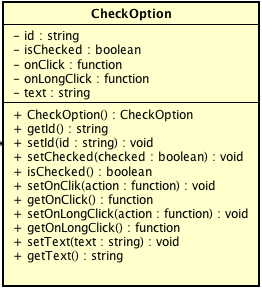
\includegraphics[scale=0.5]{Sezioni/SottosezioniST/img/CheckOption.png}
	\caption{CheckOption}
\end{figure}

\begin{itemize}
\item \textbf{Descrizione}: La classe rappresenta una entry di un widget checklist.
\item \textbf{Utilizzo}: Viene utilizzata per ogni modifica di una checklist o evento relativo ad essa, poichè gli eventi della checklist sono relativi agli opzioni che ha al suo interno.
\item \textbf{Attributi}:
	\begin{itemize}
	\item \textit{private id:string}\\
	Stringa identificativa della entry della checklist.
	\item \textit{private isChecked:boolean}\\
	Booleano che rappresenta lo stato della entry, ovvero se questa è spuntata o no.
	\end{itemize}
\item \textbf{Metodi}:
	\begin{itemize}
	\item \textit{public setChecked(checked:boolean):void}\\
	Spunta la entry o toglie la spunta da essa.
		\item{\textbf{Parametri}: \begin{itemize}
		\item \textit{checked:boolean}\\
		Il metodo spunta la entry se questo campo è true, toglie la spunta se è false.
		\end{itemize}}
	\item \textit{public boolean isChecked()}\\
	Ritorna true se la entry è spuntata, false altrimenti.
	\end{itemize}
\end{itemize}

\subsubsection{CheckStyle}

\label{CheckStyle}
\begin{figure}[ht]
	\centering
	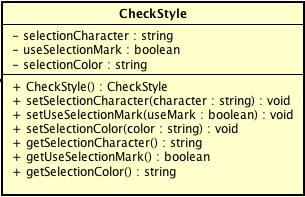
\includegraphics[scale=0.5]{Sezioni/SottosezioniST/img/CheckStyle.png}
	\caption{CheckStyle}
\end{figure}

\begin{itemize}
\item \textbf{Descrizione}: La classe rappresenta lo stile con il quale vengono indicate le spunte su una entry di una checklist.
\item \textbf{Utilizzo}: Il suo utilizzo è legato alla scelta visuale dello sviluppatore per quanto riguarda lo stile con il quale viene evidenziata una selezione nella checklist.
\item \textbf{Attributi}:
	\begin{itemize}
	\item \textit{private selectionCharacter:string}\\
	Il carattere che viene utilizzato per la spunta delle entry della checklist.
	\item \textit{private useSelectionMark:boolean}\\
	Se questo booleano è a true, le spunte verranno visualizzate con un carattere, altrimenti verranno visualizzate evidenziando le entry con un colore.
	\item \textit{private selectionColor:string}\\
	Rappresenta la stringa in esadecimale corrispondente al colore che è impostato per evidenziare le opzioni spuntate della checklist.
	\end{itemize}
\item \textbf{Metodi}:
	\begin{itemize}
	\item \textit{public setSelectionCharacter(character:string):void}\\
	Imposta il carattere per la spunta delle entry della checklist.
		\item{\textbf{Parametri}: \begin{itemize}
		\item \textit{character:string}\\
		Il carattere scelto per visualizzare le spunte.
		\end{itemize}}
	\item \textit{public setUseSelectionMark(useMark:boolean):void}\\
	Imposta l'utilizzo del carattere o del colore per evidenziare la spunta di una entry della checklist.
		\item{\textbf{Parametri}: \begin{itemize}
		\item \textit{useMark:boolean)}\\
		Se questo booleano è a true, le spunte verranno visualizzate con un carattere, altrimenti verranno visualizzate evidenziando le entry con un colore.
		\end{itemize}}
	\item \textit{public setSelectionColor(color:string):void}\\
	Imposta il colore per evidenziare le opzioni spuntate nella checklist.
		\item{\textbf{Parametri}: \begin{itemize}
		\item \textit{color:string}\\
		Rappresenta la stringa in esadecimale corrispondente al colore che verrà impostato per evidenziare le opzioni spuntate della checklist.
		\end{itemize}}
	\item \textit{public getSelectionCharacter():string}\\
	Ritorna il carattere che viene utilizzato per la spunta delle entry della checklist.
	\item \textit{public getUseSelectionMark():boolean}\\
	Ritorna true se viene utilizzato il carattere per visualizzare le spunte, altrimenti false.
	\item \textit{public getSelectionColor():string}\\
	Ritorna la stringa in esadecimale corrispondente al colore che è impostato per evidenziare le opzioni spuntate della checklist.
	\end{itemize}
\end{itemize}

\subsubsection{ListWidgetView}

\label{ListWidgetView}
\begin{figure}[ht]
	\centering
	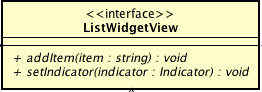
\includegraphics[scale=0.5]{Sezioni/SottosezioniST/img/ListWidgetView.png}
	\caption{ListWidgetView}
\end{figure}

\begin{itemize}
\item \textbf{Descrizione}: Questa interfaccia rappresenta la view relativa ai widget di tipo lista.
\item \textbf{Utilizzo}: L'interfaccia viene utilizzata per disaccoppiare presenter e implementazione del widget, visualizza i dati che gli vengono passati dal presenter.
\item \textbf{Attributi}:
\item \textbf{Metodi}:
	\begin{itemize}
	\item \textit{public addItem(item:string):void}\\
	Aggiunge un oggetto alla lista.
		\item{\textbf{Parametri}: \begin{itemize}
		\item \textit{item:string}\\
		Il testo dell'oggetto da aggiungere alla lista.
		\end{itemize}}
	\item \textit{public setIndicator(indicator:Indicator):void}\\
	Imposta l'indicatore per gli oggetti della lista.
		\item{\textbf{Parametri}: \begin{itemize}
		\item \textit{indicator:Indicator}\\
		Il simbolo che verrà impostato per indicare gli oggetti della lista.
		\end{itemize}}
	\end{itemize}
\end{itemize}

\subsubsection{ListWidget}

\label{ListWidget}
\begin{figure}[ht]
	\centering
	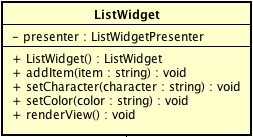
\includegraphics[scale=0.5]{Sezioni/SottosezioniST/img/ListWidget.png}
	\caption{ListWidget}
\end{figure}

\begin{itemize}
\item \textbf{Descrizione}: Questa classe rappresenta un widget lista, un elenco di oggetti senza ordine, implementando l'interfaccia ListWidgetView.
\item \textbf{Utilizzo}: Implementando i metodi di ListWidgetView questa classe viene utilizzata al momento della creazione e della personalizzazione del widget lista e del suo contenuto.
\item \textbf{Attributi}:
	\begin{itemize}
	\item \textit{private presenter:ListWidgetPresenter}\\
	Il presenter associato al widget lista, al quale questa classe delega la gestione del comportamento del widget stesso.
	\end{itemize}
\item \textbf{Metodi}:
	\begin{itemize}
	\item \textit{public addItem(item:string):void}\\
	Aggiunge un oggetto alla lista.
		\item{\textbf{Parametri}: \begin{itemize}
		\item \textit{item:string}\\
		Il testo dell'oggetto da aggiungere alla lista.
		\end{itemize}}
	\item \textit{public setIndicator(indicator:Indicator):void}\\
	Imposta l'indicatore per gli oggetti della lista.
		\item{\textbf{Parametri}: \begin{itemize}
		\item \textit{indicator:Indicator}\\
		Il simbolo che verrà impostato per indicare gli oggetti della lista.
		\end{itemize}}
	\item \textit{public renderView():string}\\
	Genera il codice HTML CSS JS necessario per visualizzare il widget.
	\end{itemize}
\end{itemize}

\subsubsection{ListWidgetPresenter}

\label{ListWidgetPresenter}
\begin{figure}[ht]
	\centering
	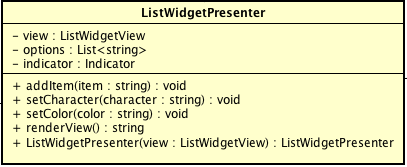
\includegraphics[scale=0.5]{Sezioni/SottosezioniST/img/ListWidgetPresenter.png}
	\caption{ListWidgetPresenter}
\end{figure}

\begin{itemize}
\item \textbf{Descrizione}: Questa classe rappresenta il presenter per i widget di tipo lista.
\item \textbf{Utilizzo}: Il presenter fa da tramite tra l'implementazione del widget e la view, formattando i dati che verranno visualizzati nella view.
\item \textbf{Attributi}:
	\begin{itemize}
	\item \textit{private view:ListWidgetView}\\
	La view associata al presenter.
	\item \textit{private options:List<string>}\\
	Questa collezione di stringhe rappresenta l'elenco di oggetti appartenenti alla lista.
	\item \textit{private indicator:Indicator}\\
	Il simbolo impostato per indicare gli oggetti della lista.
	\end{itemize}
\item \textbf{Metodi}:
	\begin{itemize}
	\item \textit{public addItem(item:string):void}\\
	Aggiunge un oggetto alla lista.
		\item{\textbf{Parametri}: \begin{itemize}
		\item \textit{item:string}\\
		Il testo dell'oggetto da aggiungere alla lista.
		\end{itemize}}
	\item \textit{public setIndicator(indicator:Indicator):void}\\
	Imposta l'indicatore per gli oggetti della lista.
		\item{\textbf{Parametri}: \begin{itemize}
		\item \textit{indicator:Indicator}\\
		Il simbolo che verrà impostato per indicare gli oggetti della lista.
		\end{itemize}}
	\item \textit{public renderView():string}\\
	Genera il codice HTML CSS JS necessario per visualizzare il widget.
	\end{itemize}
\end{itemize}

\subsubsection{Indicator}

\label{Indicator}
\begin{figure}[ht]
	\centering
	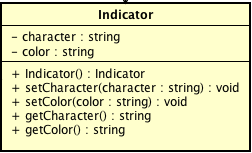
\includegraphics[scale=0.5]{Sezioni/SottosezioniST/img/Indicator.png}
	\caption{Indicator}
\end{figure}

\begin{itemize}
\item \textbf{Descrizione}: Questa classe rappresenta l'indicatore per gli oggetti di un widget lista.
\item \textbf{Utilizzo}: Ogni lista ha un indicatore per i suoi oggetti, e questa classe fornisce gli strumenti per personalizzarlo.
\item \textbf{Attributi}:
	\begin{itemize}
	\item \textit{private character:string}\\
	Il simbolo impostato per indicare gli oggetti della lista.
	\item \textit{private color:string}\\
	Rappresenta la stringa in esadecimale corrispondente al colore che è impostato per gli indicatori.
	\end{itemize}
\item \textbf{Metodi}:
	\begin{itemize}
	\item \textit{public setCharacter(character:string):void}\\
	Imposta il simbolo per indicare gli oggetti della lista.
		\item{\textbf{Parametri}: \begin{itemize}
		\item \textit{character:string}\\
		Il simbolo che verrà impostato per indicare gli oggetti della lista.
		\end{itemize}}
	\item \textit{public setColor(color:string):void}\\
	Imposta il colore degli indicatori.
		\item{\textbf{Parametri}: \begin{itemize}
		\item \textit{color:string}\\
		la stringa in esadecimale corrispondente al colore che verrà impostato per gli indicatori.
		\end{itemize}}
	\item \textit{public getCharacter():string}\\
	Ritorna il simbolo usato per indicare gli oggetti della lista.
	\item \textit{public getColor():string}\\
	Ritorna la stringa in esadecimale corrispondente al colore che è impostato per gli indicatori.
	\end{itemize}
\end{itemize}

\subsubsection{ImageWidgetView}

\label{ImageWidgetView}
\begin{figure}[ht]
	\centering
	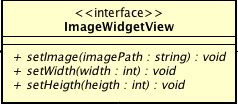
\includegraphics[scale=0.5]{Sezioni/SottosezioniST/img/ImageWidgetView.png}
	\caption{ImageWidgetView}
\end{figure}

\begin{itemize}
\item \textbf{Descrizione}: Questa interfaccia rappresenta la view relativa ai widget di tipo immagine.
\item \textbf{Utilizzo}: L'interfaccia viene utilizzata per disaccoppiare presenter e implementazione del widget.
\item \textbf{Attributi}:
\item \textbf{Metodi}:
	\begin{itemize}
	\item \textit{public setImage(imagePath:string):void}\\
	Imposta il percorso nel file system che porta all'immagine che si vuole inserire nel widget.
		\item{\textbf{Parametri}: \begin{itemize}
		\item \textit{imagePath:string}\\
		Il percorso dell'immagine.
		\end{itemize}}
	\item \textit{public setHeight(height:int):void}\\
	Imposta l'altezza dell'immagine.
		\item{\textbf{Parametri}: \begin{itemize}
		\item \textit{height:int}\\
		L'altezza dell'immagine che si vuole impostare.
		\end{itemize}}
	\item \textit{public setWidth(width:int):void}\\
	Imposta la larghezza dell'immagine.
		\item{\textbf{Parametri}: \begin{itemize}
		\item \textit{width:int}\\
		La larghezza dell'immagine che si vuole impostare.
		\end{itemize}}
	\end{itemize}
\end{itemize}

\subsubsection{ImageWidget}

\label{ImageWidget}
\begin{figure}[ht]
	\centering
	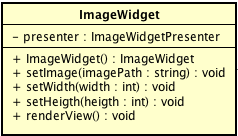
\includegraphics[scale=0.5]{Sezioni/SottosezioniST/img/ImageWidget.png}
	\caption{ImageWidget}
\end{figure}

\begin{itemize}
\item \textbf{Descrizione}: Questa classe rappresenta un widget immagine, implementando l'interfaccia ImageWidgetView.
\item \textbf{Utilizzo}: Implementando i metodi di ImageWidgetView questa classe viene utilizzata al momento della creazione e della personalizzazione del widget immagine e del suo contenuto.
\item \textbf{Attributi}:
	\begin{itemize}
	\item \textit{private presenter:ImageWidgetPresenter}\\
	Il presenter associato al widget immagine, al quale questa classe delega la gestione del comportamento del widget stesso.
	\end{itemize}
\item \textbf{Metodi}:
	\begin{itemize}
	\item \textit{public setImage(imagePath:string):void}\\
	Imposta il percorso nel file system che porta all'immagine che si vuole inserire nel widget.
		\item{\textbf{Parametri}: \begin{itemize}
		\item \textit{imagePath:string}: Il percorso dell'immagine.
		\end{itemize}}
	\item \textit{public setHeight(height:int):void}\\
	Imposta l'altezza dell'immagine.
		\item{\textbf{Parametri}: \begin{itemize}
		\item \textit{height:int}\\
		L'altezza dell'immagine che si vuole impostare.
		\end{itemize}}
	\item \textit{public setWidth(width:int):void}\\
	Imposta la larghezza dell'immagine.
		\item{\textbf{Parametri}: \begin{itemize}
		\item \textit{width:int}\\
		La larghezza dell'immagine che si vuole impostare.
		\end{itemize}}
	\item \textit{public renderView():string}\\
	Genera il codice HTML CSS JS necessario per visualizzare il widget.
	\end{itemize}
\end{itemize}

\subsubsection{ImageWidgetPresenter}

\label{ImageWidgetPresenter}
\begin{figure}[ht]
	\centering
	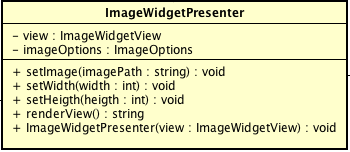
\includegraphics[scale=0.5]{Sezioni/SottosezioniST/img/ImageWidgetPresenter.png}
	\caption{ImageWidgetPresenter}
\end{figure}

\begin{itemize}
\item \textbf{Descrizione}: Questa classe rappresenta il presenter per i widget di tipo lista.
\item \textbf{Utilizzo}: Il presenter fa da tramite tra l'implementazione del widget e la view, formattando i dati che verranno visualizzati nella view.
\item \textbf{Attributi}:
	\begin{itemize}
	\item \textit{private view:ImageWidgetView}\\
	La view associata al presenter.
	\item \textit{private imageOptions:ImageOptions}\\
	Contiene le impostazioni attuali del widget.
	\end{itemize}
\item \textbf{Metodi}:
	\begin{itemize}
	\item \textit{public setImage(imagePath:string):void}\\
	Imposta il percorso nel file system che porta all'immagine che si vuole inserire nel widget.
		\item{\textbf{Parametri}: \begin{itemize}
		\item \textit{imagePath:string}\\
		Il percorso dell'immagine.
		\end{itemize}}
	\item \textit{public setHeight(height:int):void}\\
	Imposta l'altezza dell'immagine.
		\item{\textbf{Parametri}: \begin{itemize}
		\item \textit{height:int}\\
		L'altezza dell'immagine che si vuole impostare.
		\end{itemize}}
	\item \textit{public setWidth(width:int):void}\\
	Imposta la larghezza dell'immagine.
		\item{\textbf{Parametri}: \begin{itemize}
		\item \textit{width:int}\\
		La larghezza dell'immagine che si vuole impostare.
		\end{itemize}}
	\item \textit{public renderView():string}\\
	Genera il codice HTML CSS JS necessario per visualizzare il widget.
	\end{itemize}
\end{itemize}

\subsubsection{ImageOptions}

\label{ImageOptions}
\begin{figure}[ht]
	\centering
	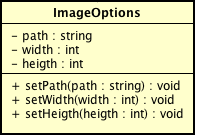
\includegraphics[scale=0.5]{Sezioni/SottosezioniST/img/ImageOptions.png}
	\caption{ImageOptions}
\end{figure}

\begin{itemize}
\item \textbf{Descrizione}: Questa classe rappresenta le impostazioni di un widget immagine.
\item \textbf{Utilizzo}: Ogni cambiamento delle impostazioni di visualizzazione di un widget immagine coinvolge questa classe.
\item \textbf{Attributi}:
	\begin{itemize}
	\item \textit{private path:string}\\
	Il percorso dell'immagine.
	\item \textit{private width:int}\\
	L'altezza dell'immagine. 
	\item \textit{private height:int}\\
	La larghezza dell'immagine. 
	\end{itemize}
\item \textbf{Metodi}:
	\begin{itemize}
	\item \textit{public setPath(path:string):void}\\
	Imposta il percorso nel file system che porta all'immagine che si vuole inserire nel widget.
		\item{\textbf{Parametri}: \begin{itemize}
		\item \textit{path:string}\\
		Il percorso dell'immagine.
		\end{itemize}}
	\item \textit{public setHeight(height:int):void}\\
	Imposta l'altezza dell'immagine.
		\item{\textbf{Parametri}: \begin{itemize}
		\item \textit{height:int}\\
		L'altezza dell'immagine che si vuole impostare.
		\end{itemize}}
	\item \textit{public setWidth(width:int):void}\\
	Imposta la larghezza dell'immagine.
		\item{\textbf{Parametri}: \begin{itemize}
		\item \textit{width:int}\\
		La larghezza dell'immagine che si vuole impostare.
		\end{itemize}}
	\end{itemize}
\end{itemize}